% !TEX root = ../main.tex
\section{User Interface}\label{sec:user-interface}
% Initial designs
Some initial designs were created for user interfaces for features that had been planned, these included jump tracking, landing pattern planner, jump stats review and a settings menu. Each feature had several different designs. Eight people were asked to pick their favourite of the designs for each feature and also comment on what improvements could be made or which aspects of other designs they would like to see brought into the app.

Figure~\vref{fig:app-designs} shows several of the designs that were created and shown to participants providing feedback including both skydivers and non-skydivers.

\begin{figure}[ht]
  \centering
  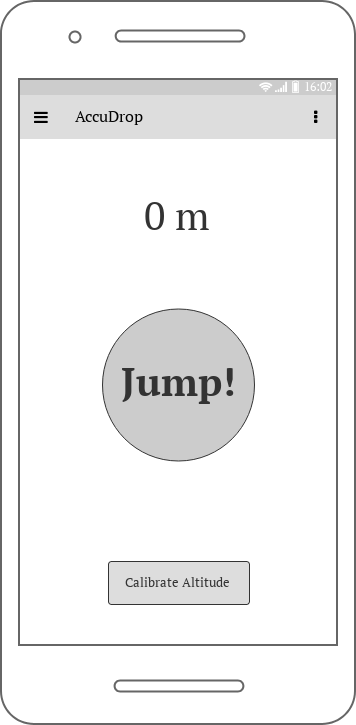
\includegraphics[width=0.2\linewidth]{jump-design}
  \hspace{1cm}
  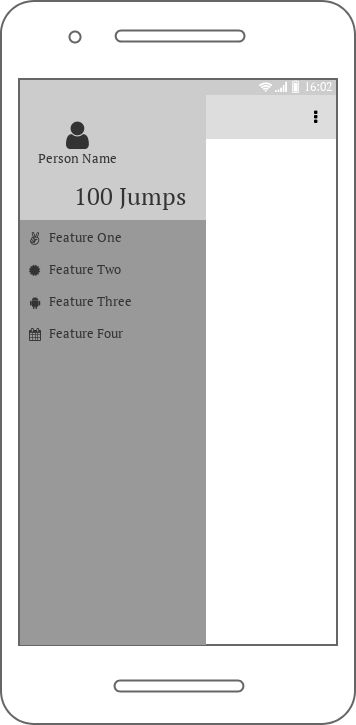
\includegraphics[width=0.2\linewidth]{menu-design}
  \hspace{1cm}
  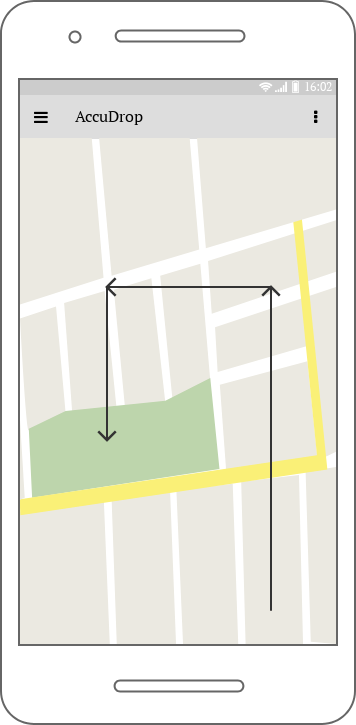
\includegraphics[width=0.2\linewidth]{pattern-design}

  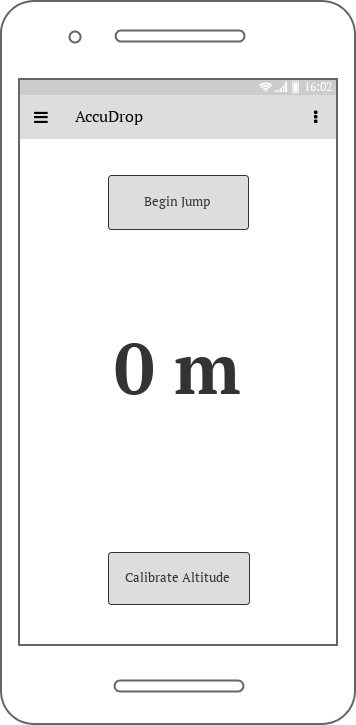
\includegraphics[width=0.2\linewidth]{jump-design-alt}
  \hspace{1cm}
  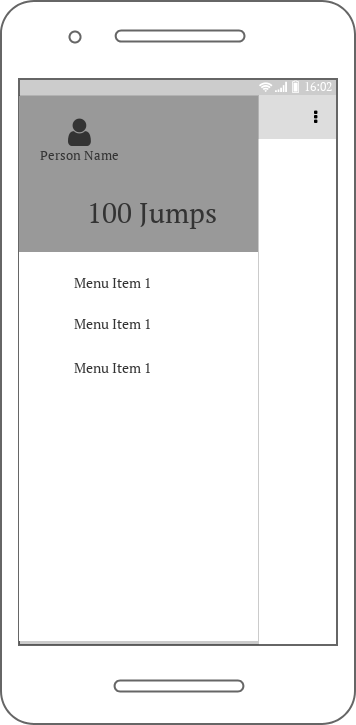
\includegraphics[width=0.2\linewidth]{menu-design-alt}
  \hspace{1cm}
  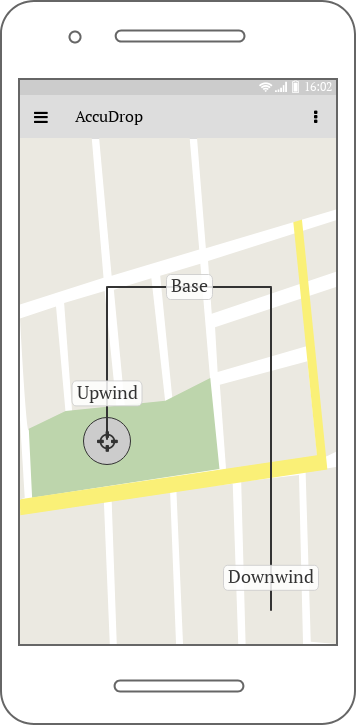
\includegraphics[width=0.2\linewidth]{pattern-design-alt}
  \caption{Initial app design variations.}\label{fig:app-designs}
\end{figure}

With input from the feedback participants, final designs were decided from the list of initial designs, with small adjustments based on the participants comments.

\subsection{The Interface}
When implementing the interface of the app, we tried to follow the Android style guides wherever possible. Interface design/implementation didn't always necessarily take priority or go through rigorous procedures since the main objective of the project was to fulfil the proof of concept objectives rather than create a product for skydivers.

% App Icon
An app icon was created that clearly reflects the subject of the app, with a scalable SVG parachutist image in the centre. The whole icon is simple, scalable and allows for Android to adjust the size and shape depending on which version of the OS is being used. The icon that was created for Android Oreo can be seen in Figure~\vref{fig:icon}.

\begin{wrapfigure}{l}{0.25\textwidth}
  \centering
  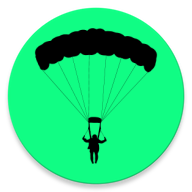
\includegraphics[width=0.2\textwidth]{icon}
  \caption{The app icon for Android Oreo.}\label{fig:icon}
\end{wrapfigure}

% Splash screen
Loading an app can occasionally take a long time on slower systems, Android recommends that the first screen to be loaded by the phone is a splash screen that does not contain any logic other than loading the rest of the app. The splash screen ensures that a user is aware that the app has been started and does not attempt to interact with main elements of the app that may not be loaded to work correctly yet. The splash screen follows the green colour scheme of the app and shows the app icon in the centre, this can be seen in Figure~\vref{fig:splash}.

\begin{wrapfigure}[21]{l}{0.3\textwidth}
  \centering
  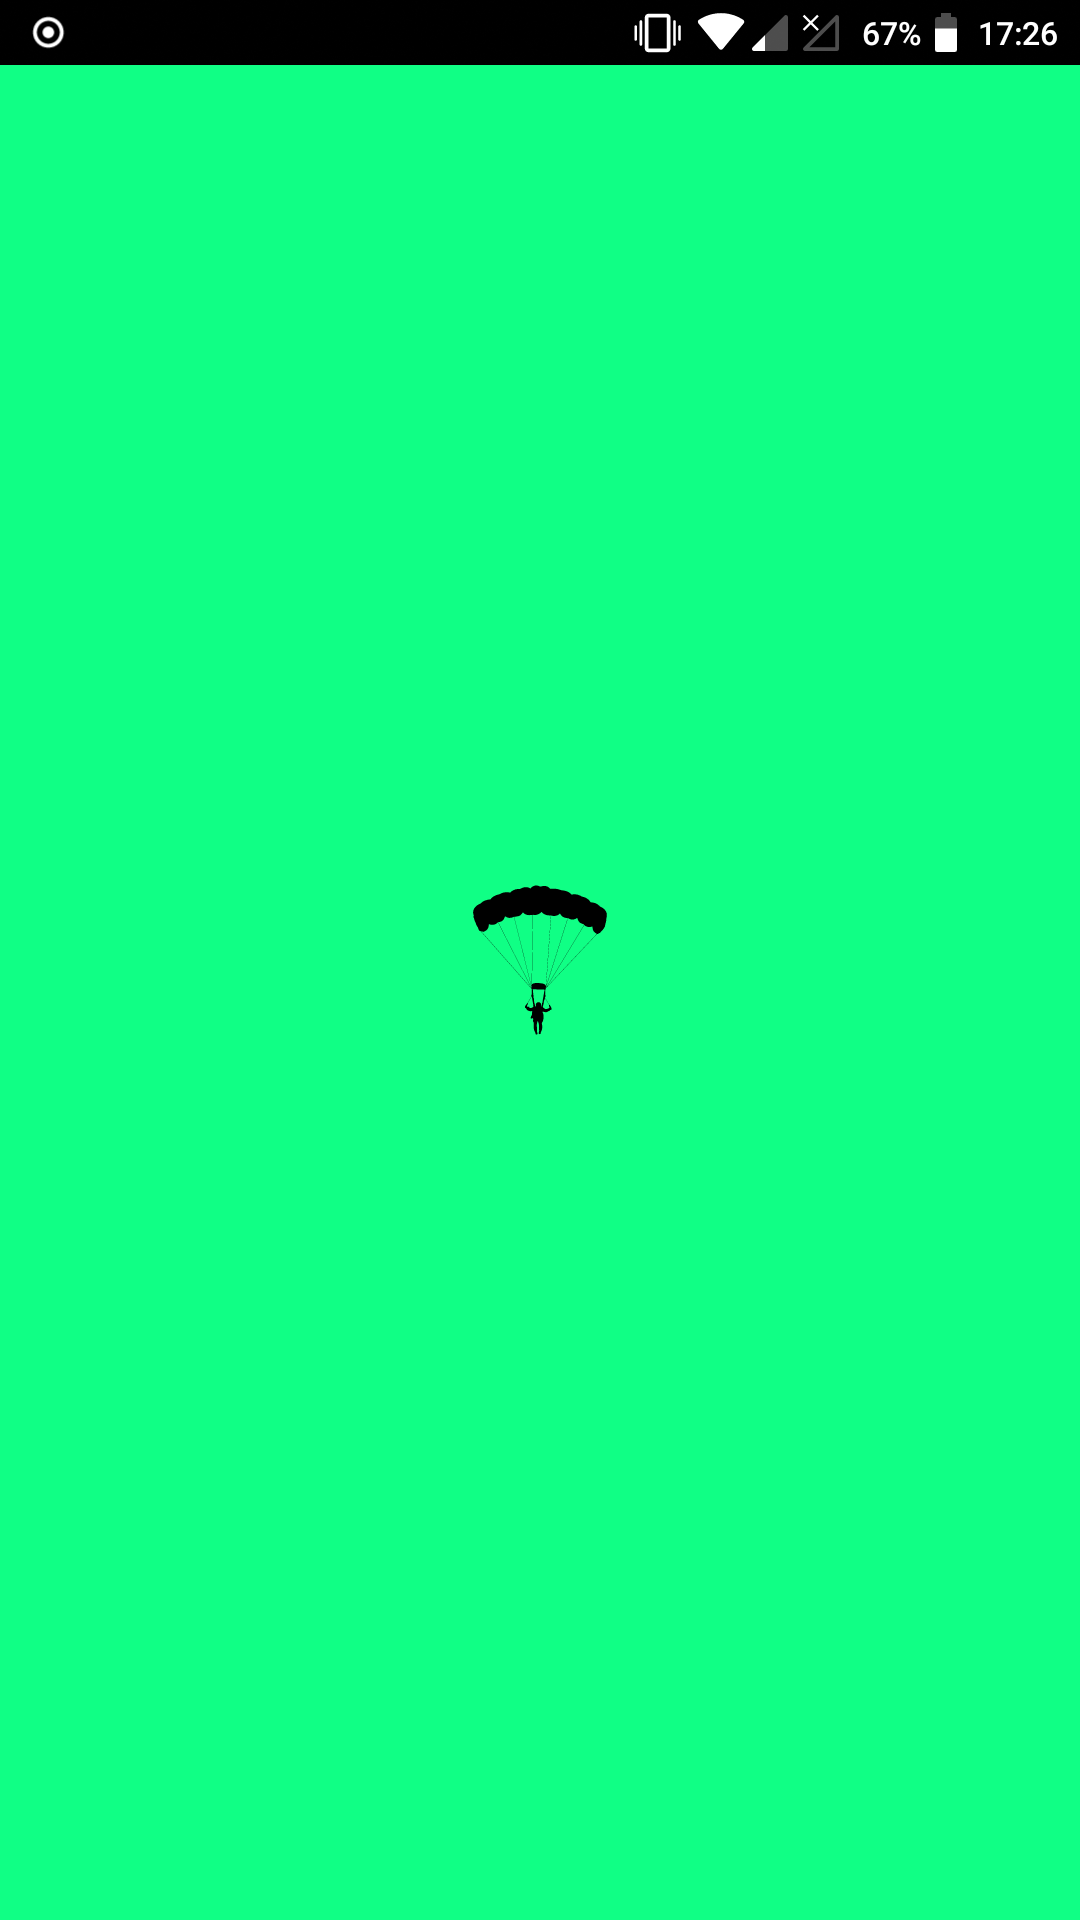
\includegraphics[width=0.3\textwidth]{splash-scrot}
  \caption{The app startup splash screen.}\label{fig:splash}
\end{wrapfigure}

% Landing Pattern Planner
The landing pattern planner feature's user interface was implemented very similarly to the initial designs. Figure~\vref{fig:planner} shows a screenshot of the app with the feature in use. Google Maps look great in Android and are easily added to a screen. Most people are already familiar with Google Maps on mobile and so are able to use the familiar controls to manipulate the map.

The user is able to hold down on a location to set their target landing area. While weather data and landing patterns are being generated, a progress bar will show at the top of the screen to indicate that the app is working on their request. Typically, the app will finish the landing pattern generation quickly and so the progress bar is not required. One major difference from the original designs for the interface is that map markers are used at each turn point. The map markers are used to allow the user to interact with the route to see the altitudes of each turn. The colour red is used for the route's line overlays since this is easily visible on most dropzone map areas which are typically mostly green.

\begin{wrapfigure}{L}{0.3\textwidth}
  \centering
  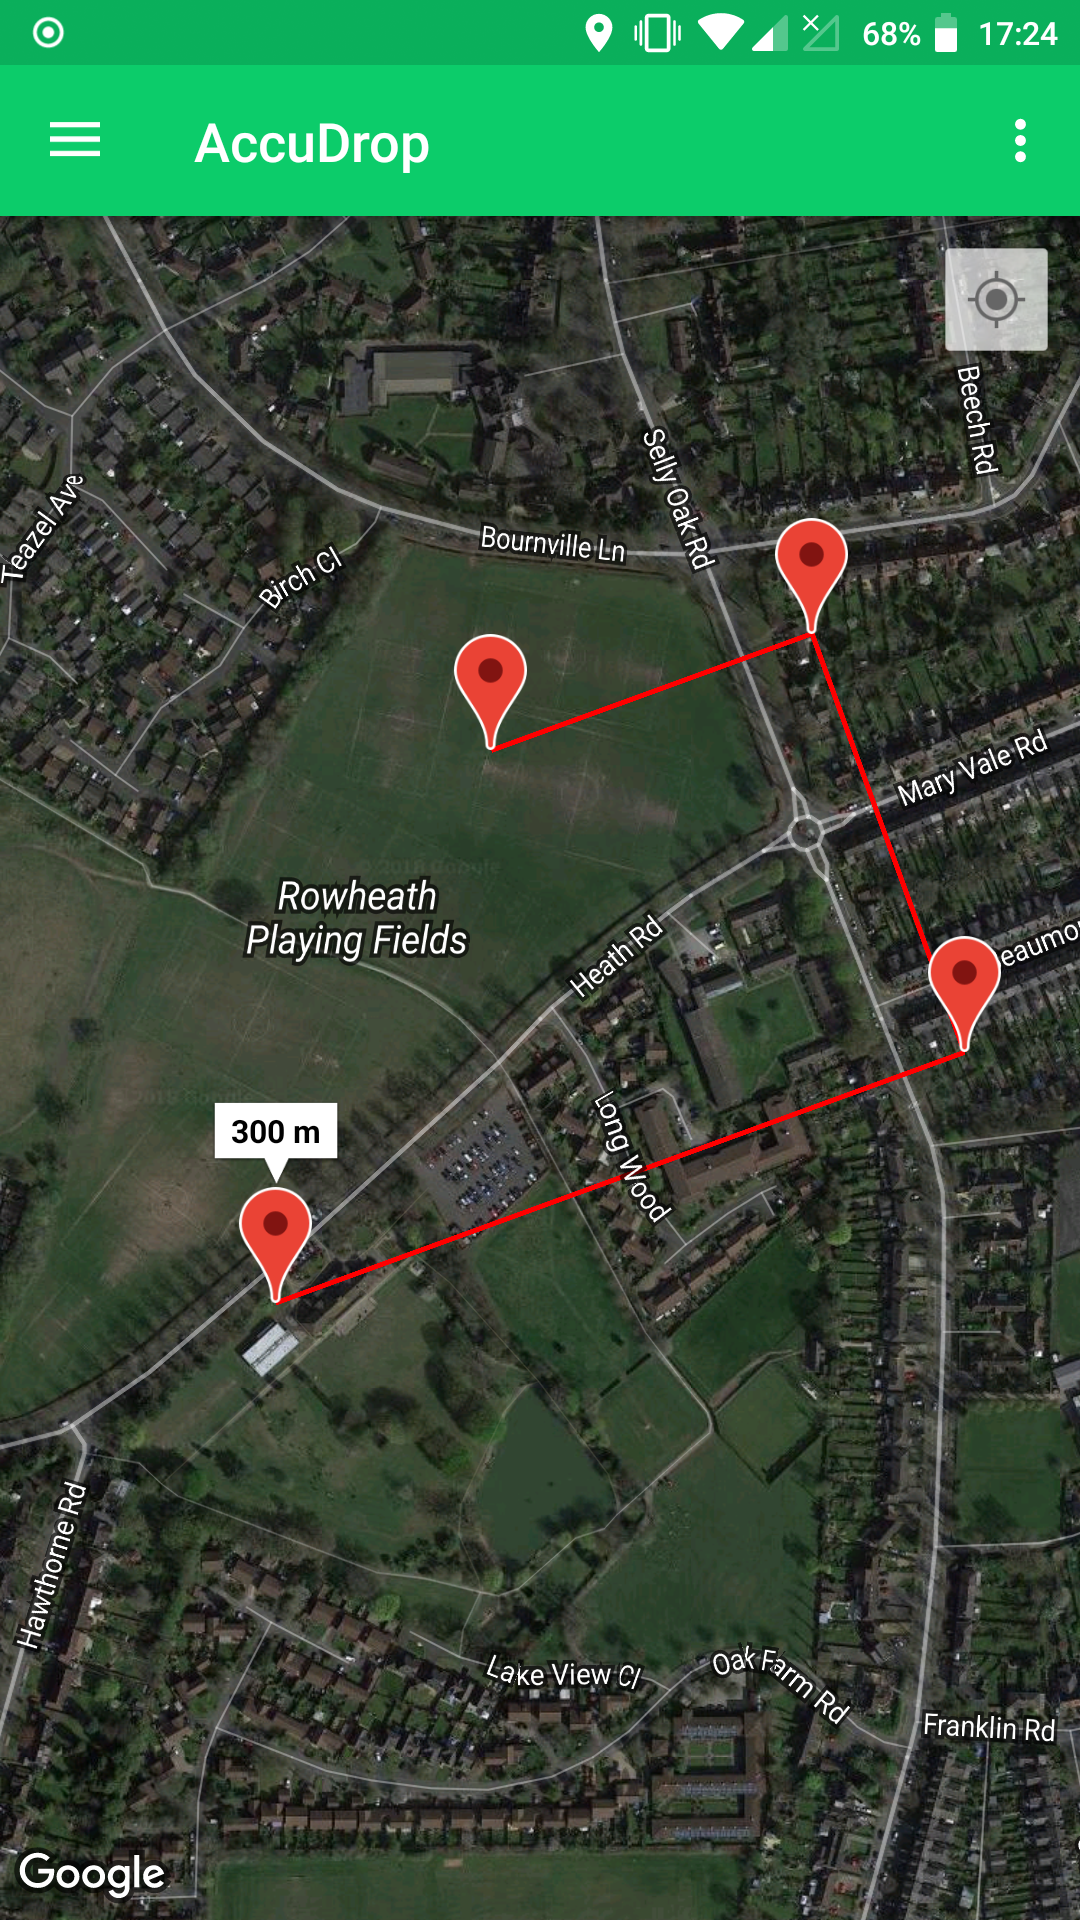
\includegraphics[width=0.3\textwidth]{planner-scrot}
  \caption{The landing pattern planner screen.}\label{fig:planner}
\end{wrapfigure}

% Jump Stats
The jump statistics screen is simple, values for different statistics are displayed in text form. Each statistic value is updated once the value has been fetched, the UI never hangs while waiting for data. At the bottom of the screen there are buttons to switch move between different jumps, as these buttons are used, the large jump number at the top of the display and all of the statistics are updated. The screen will adapt to rotation, providing a different layout that still allows for all of the data to be displayed on the screen. Arrows indicate the difference between speed statistics, with a down arrow indicating fall rate and a right arrow indicating horizontal speed.

The choice was made to keep jump statistics separate from jump data replay features such as landing pattern and freefall review to keep the interface simple and easy to use for a user, rather than requiring swiping gestures to scroll etc.
The jump statistics UI can be seen Figure~\ref{fig:stats}.

\begin{wrapfigure}{r}{0.3\textwidth}
  \centering
  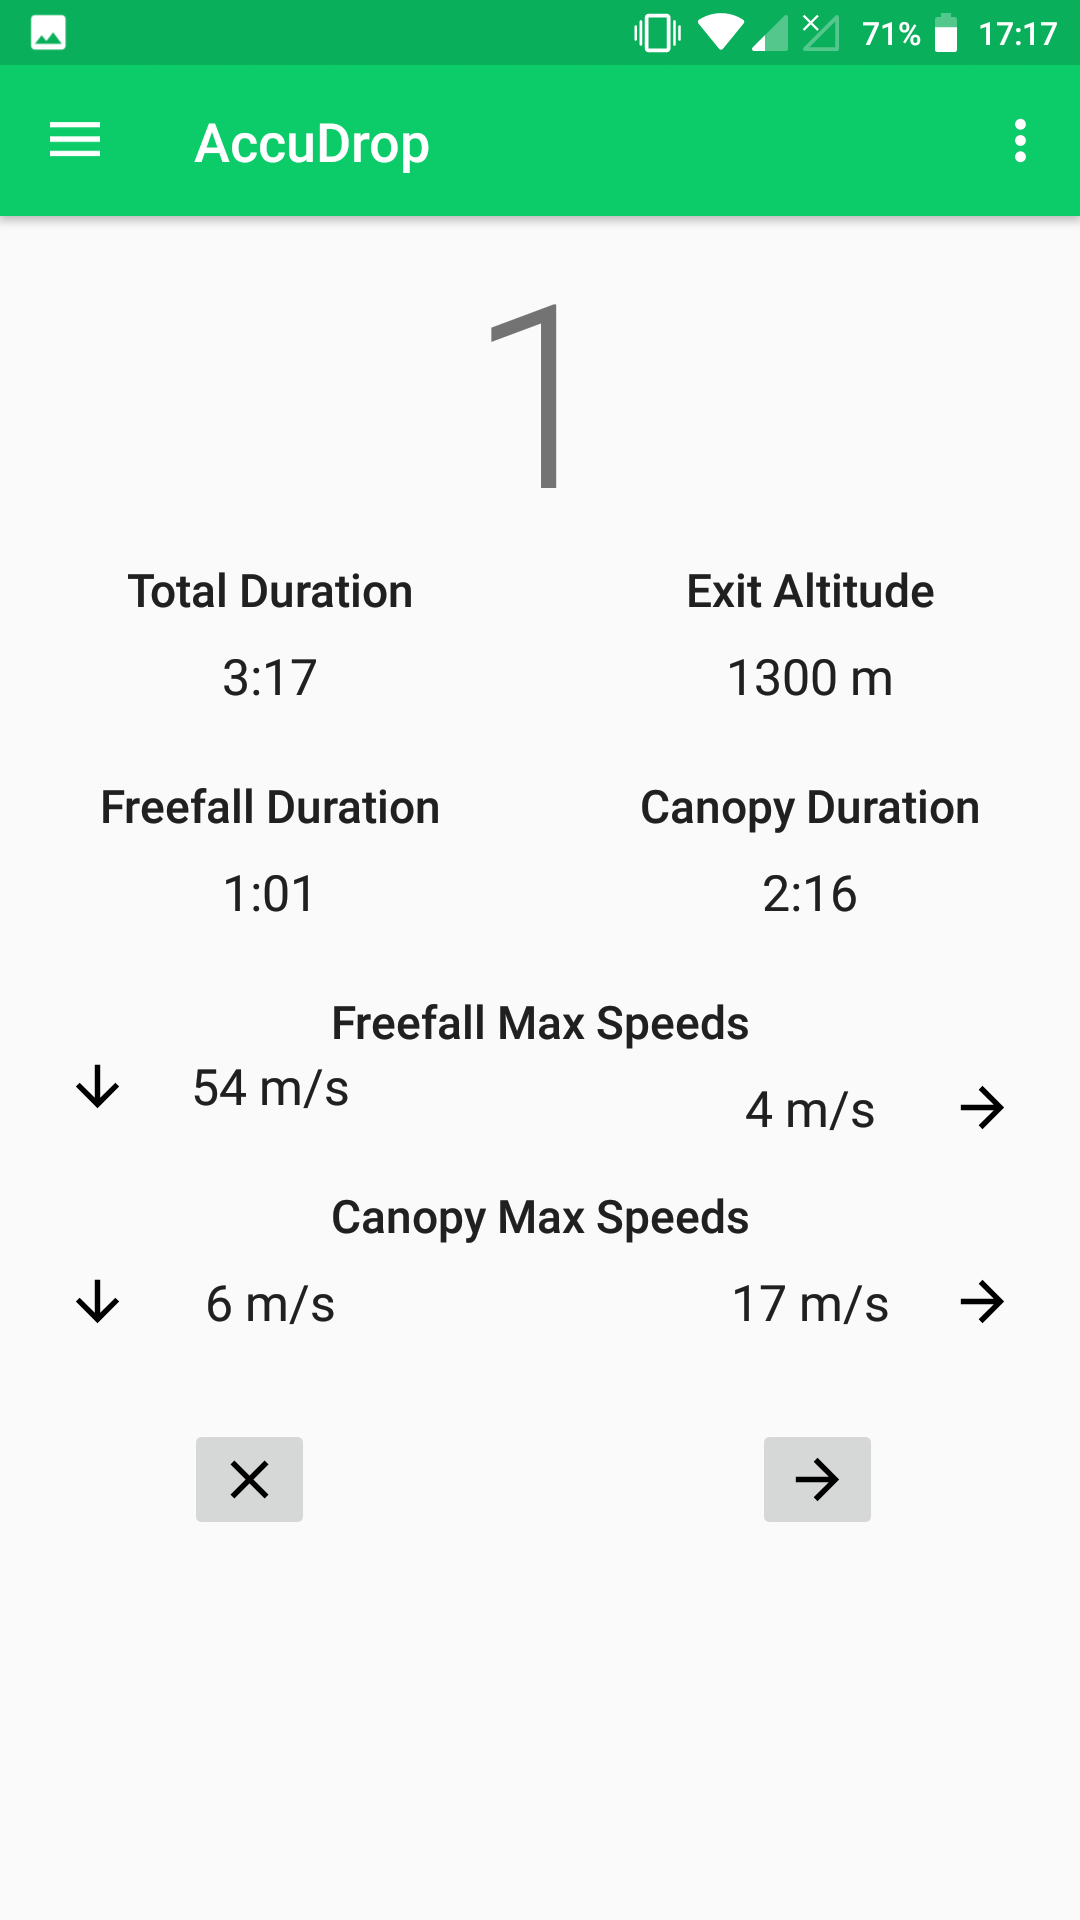
\includegraphics[width=0.3\textwidth]{stats-scrot}
  \caption{The jump statistics screen.}\label{fig:stats}
\end{wrapfigure}

% Landing Pattern Viewer
The landing pattern viewer is designed to match the landing pattern planner screen. A Google Map is used that the logged positional data from a jump is overlayed onto. Since Google Map overlays cannot be positioned using 3D coordinates, the screen is split into two parts. The second part of the screen is used to show how altitude data compares to horizontal movement in the landing pattern data.

The perpendicular view of the landing pattern can be altered, to change the direction from which the pattern is being looked at, this is done by rotating the Google Map. The perpendicular view represents a view in the direction from the bottom of the Google Map to the top.

The perpendicular view is not very intuitive to understand. Improvements could be made by redesigning or adding a side-scrolling sky view to indicate which way the view is moving. Alternatively, more advanced graphical technology could be used to present the landing pattern in a three dimensional view. Unfortunately, time was not available for these improvements to be made.

The landing pattern viewer display can be seen in Figure~\ref{fig:landing-scrot}.


% Freefall Radar View
The freefall radar view (shown in Figure~\vref{fig:radar}) was not designed before the implementation, the feature was based on the radar from old X-Wing computer games. The view shows radar view shown as an ellipse to simulate it being looked at from an angle. A subject is positioned in the middle of the screen as a dot with many other dots around them representing other skydivers' positions. A line from the radar plane to each dot indicates the altitude difference of each skydiver from the subject user's altitude.

Different subject skydivers can be selected by simply touch one of the dots, each dot's identity can be identified by a small label giving the skydiver's name. To avoid the view being cluttered by lines of skydivers that are very far from the subject, if a skydiver's position would be drawn off the screen, the position is not drawn.

Buttons allow for a user to switch between different jumps, and a seek bar allows for the user to easily move through a position in time for the jump data. The controls for this feature are simple are simple and intuitive to use. When given to a user to test the feature, they had no problems in using the controls without direction, what they did occasionally not understand was what the lines from each skydiver's position indicated. Given more time, a key could be added to the view to indicate the meaning of the lines.

% Settings
Android has a lot of guidelines for settings windows, as well as templates that can be generated in their IDE, Android Studio. Guidelines and templates were used to organise and design a settings screen that appears to be very similar to a typical Android operating system settings screen.
The settings screen that created is included in Figure~\vref{fig:settings}.

\begin{figure}[ht]
  \centering
  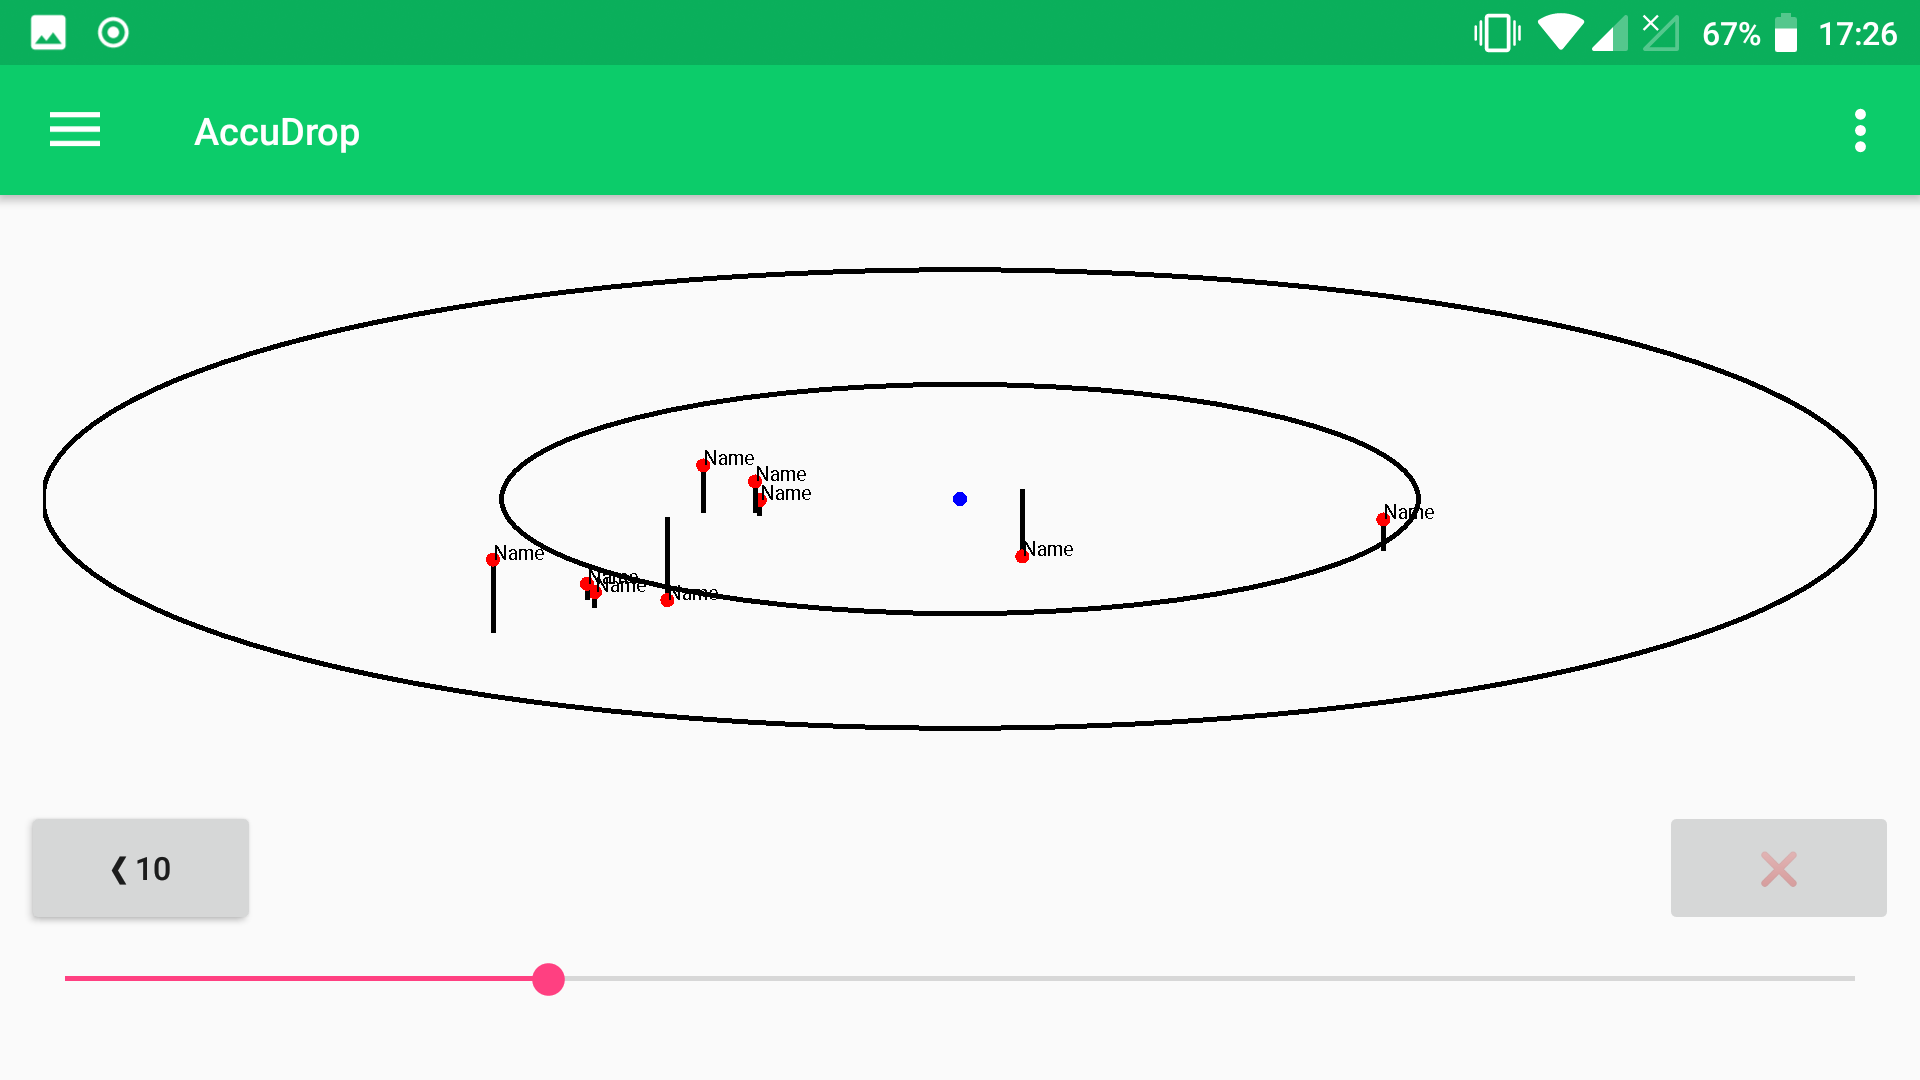
\includegraphics[width=\textwidth]{radar-scrot}
  \caption{The freefall formation skydiving radar view feature.}\label{fig:radar}
\end{figure}

\begin{figure}[H]
\centering
\begin{minipage}{.5\textwidth}
    \centering
    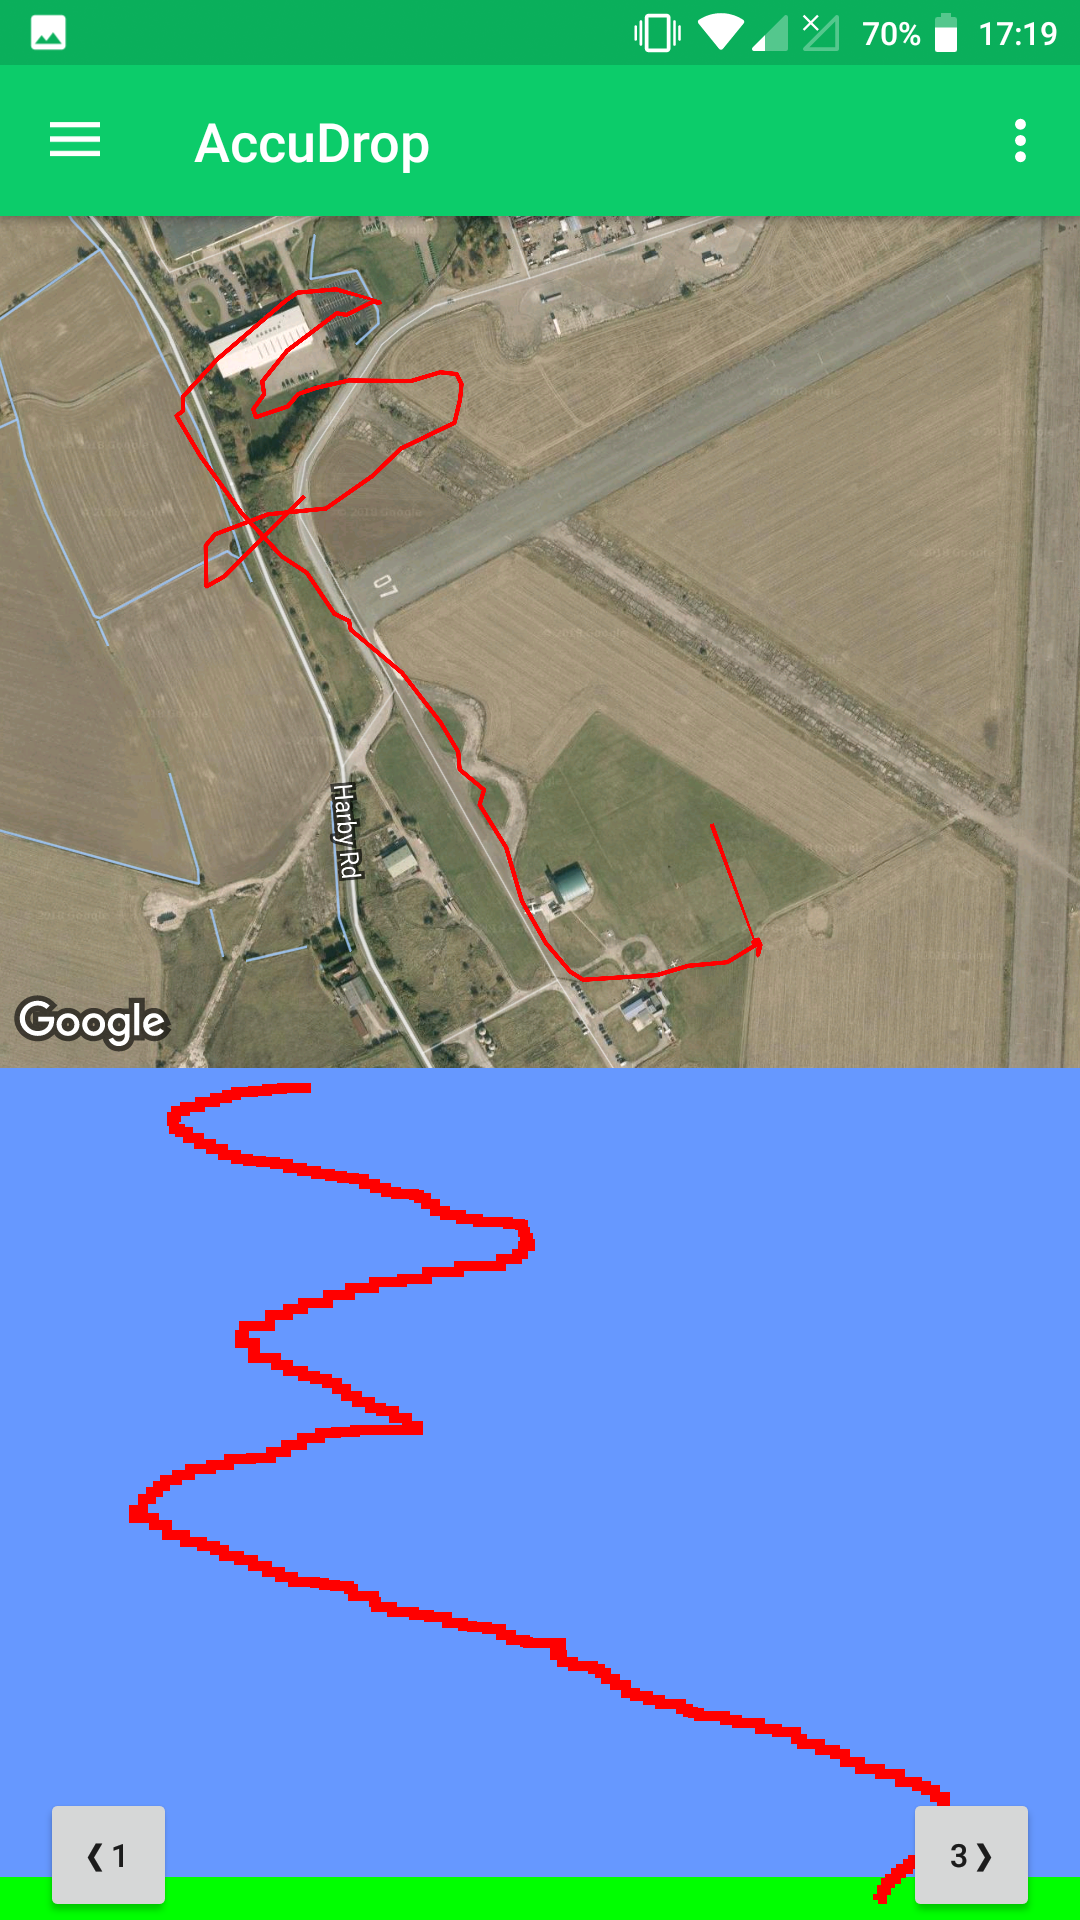
\includegraphics[width=0.9\linewidth]{landing-scrot}
    \captionof{figure}{The landing pattern viewer feature.}\label{fig:landing-scrot}
\end{minipage}%
\begin{minipage}{.5\textwidth}
    \centering
    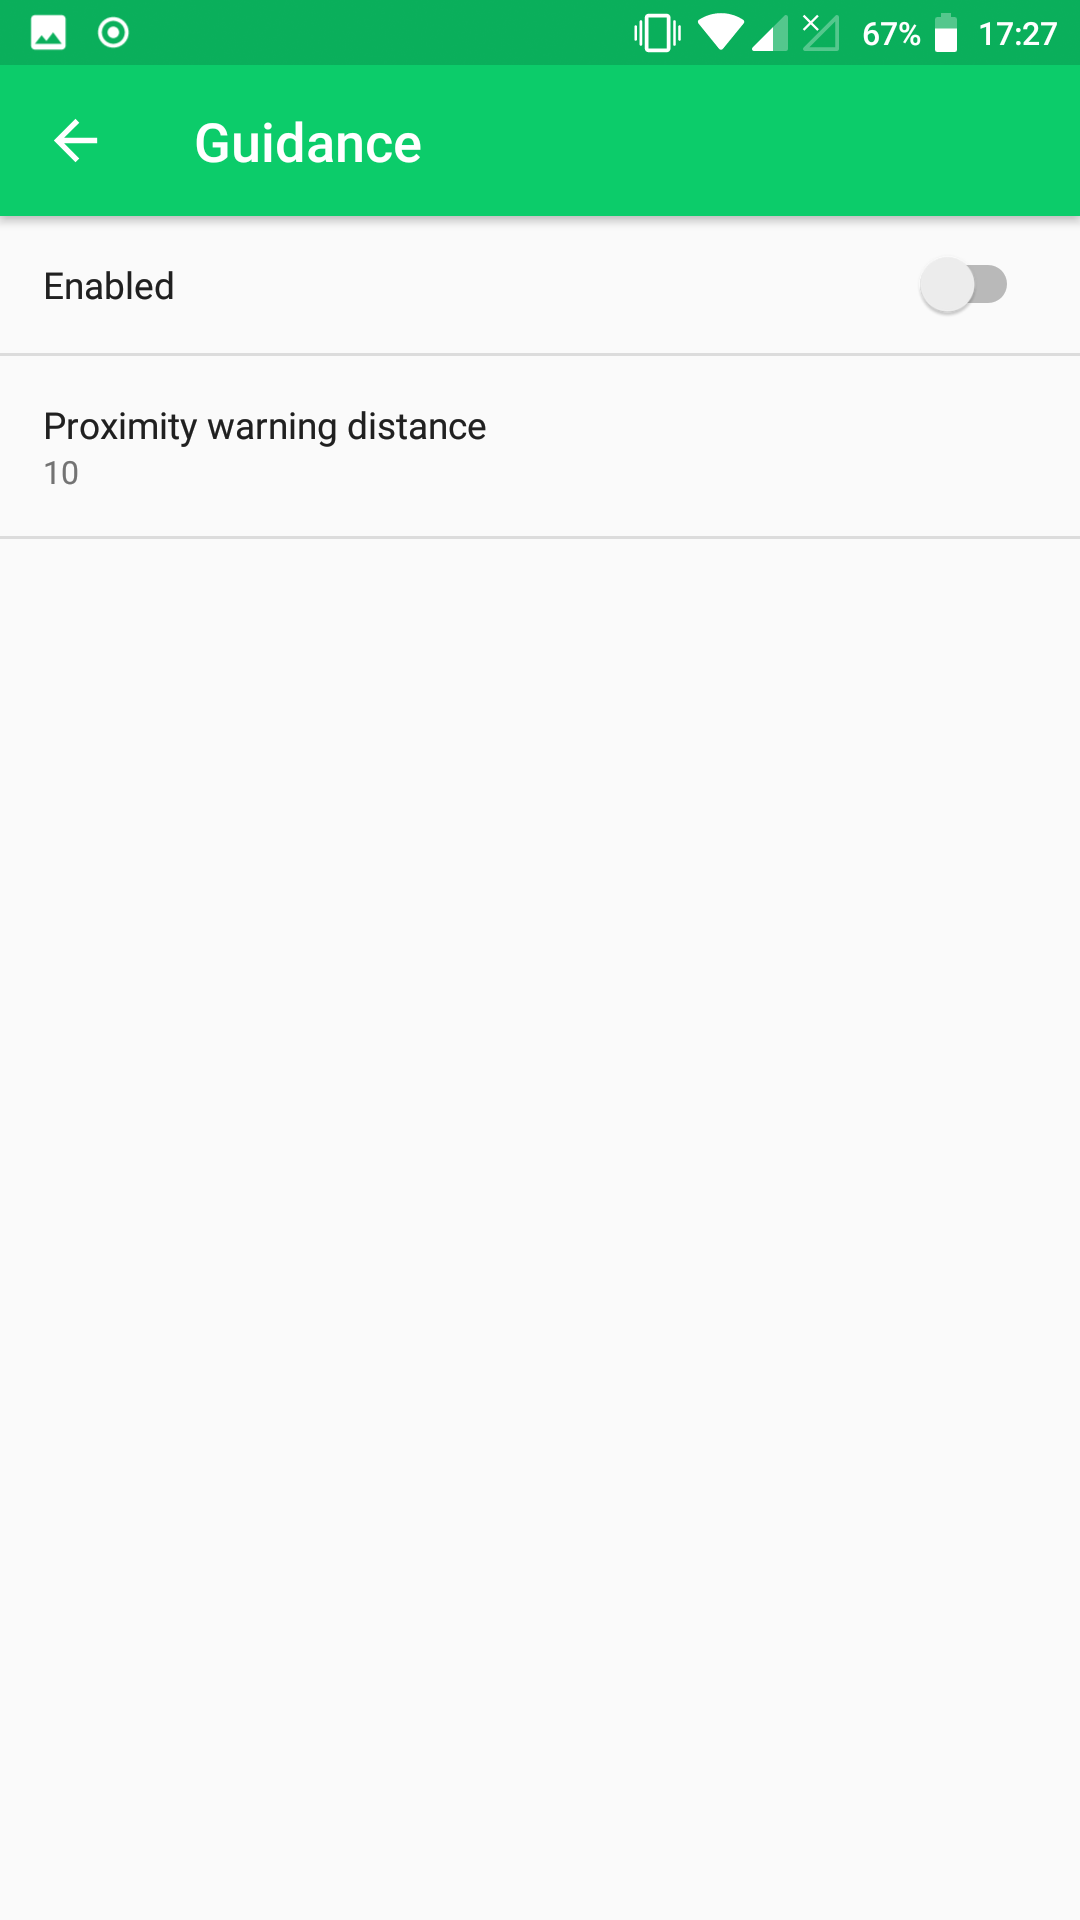
\includegraphics[width=0.9\linewidth]{settings-scrot}
    \captionof{figure}{The settings screen for the app.}\label{fig:settings}
\end{minipage}
\end{figure}
